\documentclass[conference]{IEEEtran}
\usepackage[T1]{fontenc}
\usepackage{cite}
\usepackage{amsmath,amssymb}
\usepackage{graphicx}
\usepackage{booktabs}
\usepackage{array}
\usepackage{url}
\usepackage{hyperref}
\graphicspath{{figures/}}
\hypersetup{colorlinks=true,linkcolor=black,citecolor=black,urlcolor=blue}

\begin{document}

\title{Deep Convolutional Neural Networks on Fashion-MNIST:\\ Breaking the Handcrafted Spatial Ceiling with Global Average Pooling\\ (Phase 2 --- Deep-Learning Evaluation)}

\author{\IEEEauthorblockN{MD. Sajjan, Sibtain Ahmed Qureshi, Syed Darain Qamar, Antik Mandal, Abuzar Haideri}
\IEEEauthorblockA{Department of CS/AI\\
Newton School of Technology\\
Course: Advanced Machine Learning}}

\maketitle

\begin{abstract}
In Phase~1, classical classifiers evaluated on Fashion-MNIST with handcrafted Histogram of Oriented Gradients (HOG) features reached a performance plateau of 91.30\% test accuracy (RBF Support Vector Machine), with 60--65\% of remaining errors trapped inside the ambiguous upper-body garment cluster \{T-shirt, Pullover, Coat, Shirt\}. This Phase~2 report investigates whether end-to-end learnable convolutional representations can resolve this fine-grained ambiguity under an identical, leak-free protocol (48{,}000 train, 12{,}000 validation, 10{,}000 test; seed 42). We design and benchmark a 2-block baseline ConvNet (with and without data augmentation) and a modernized 3-block architecture incorporating Global Average Pooling (CNN3Block-GAP). We explicitly analyze why candidate alternatives---such as pre-trained ImageNet models (ResNet/VGG), Vision Transformers (ViT), and deep Multi-Layer Perceptrons---were rejected due to severe resolution mismatch ($28\times28$ vs.\ $224\times224$), lack of 2D inductive bias, or extreme overparameterization. Our best architecture, CNN3Block-GAP, achieves 93.09\% test accuracy and 0.9306 macro-F1, delivering a statistically definitive improvement over the best classical SVM (McNemar $\chi^2 = 44.56, p = 2.46 \times 10^{-11}$). Total test errors fall from 870 to 691, with Pullover recall increasing from 0.856 to 0.906 and Coat recall rising from 0.875 to 0.924. Concurrently, Global Average Pooling reduces model storage by $60\times$ (304{,}682 weights vs.\ 18.1M support vectors) and accelerates CPU inference to 0.68~ms/image ($8\times$ faster). Grad-CAM saliency maps confirm that convolutional feature maps localize discriminating collar and hemline contours that fixed HOG grids fail to resolve.
\end{abstract}

\begin{IEEEkeywords}
Fashion-MNIST, Convolutional Neural Networks, Global Average Pooling, Grad-CAM, McNemar Test, Model Selection, Error Analysis.
\end{IEEEkeywords}

\section{Introduction}
Fashion-MNIST~\cite{xiao2017} was introduced as a challenging drop-in replacement for the digit MNIST benchmark~\cite{lecun1998}, presenting 70{,}000 $28\times28$ grayscale images across 10 balanced garment categories. In Phase~1, our study isolated the effect of fixed spatial descriptors (HOG) on classical learners (Logistic Regression, $k$-NN, Random Forest, and RBF-SVM). While HOG yielded significant improvements over flattened raw pixels for linear and kernel models, performance saturated at 91.30\% (SVM-RBF), leaving an unresolved error cluster where Shirt recall reached only 0.750.

\textbf{Phase~2 Objective.} Phase~2 investigates deep learning architectures trained end-to-end directly on 2D pixel grids. We seek to determine:
\begin{enumerate}
\item Can learned spatial filters break the 91.30\% classical ceiling?
\item Does increasing network depth and replacing fully connected layers with Global Average Pooling (GAP) prevent overfitting while expanding effective receptive field?
\item How do CNNs compare with classical ML on computational footprint (parameters) and single-image CPU latency?
\end{enumerate}

\section{Architectural Selection and Rejected Alternates}
A critical requirement in deep learning engineering is justifying why specific architectures were adopted while popular alternatives were excluded.

\subsection{Architectures Evaluated}
\textbf{1. CNN2Block (Baseline):} Two stages of $[\mathrm{Conv}(3\times3, 32/64) \to \mathrm{BN} \to \mathrm{ReLU} \to \mathrm{MaxPool}(2\times2)]$ followed by $\mathrm{Flatten} \to \mathrm{Linear}(3136, 128) \to \mathrm{ReLU} \to \mathrm{Dropout}(0.4) \to \mathrm{Linear}(10)$. Total parameters: 421{,}738.

\textbf{2. CNN2Block+Aug:} Identical to CNN2Block but trained with spatial augmentations (random horizontal flip $p=0.5$ and random crop with 2-px reflection padding).

\textbf{3. CNN3Block-GAP (Best Model):} Three double-convolution stages (channels 32, 64, 128) with batch normalisation and max-pooling, terminated by Global Average Pooling ($\mathrm{AdaptiveAvgPool2d}((1, 1))$) and a compact classifier ($\mathrm{Linear}(128, 128) \to \mathrm{Dropout}(0.3) \to \mathrm{Linear}(10)$). Eliminating the high-dimensional flattening layer reduces parameters to \textbf{304{,}682} while tripling feature depth.

\subsection{Why Candidate Alternatives Were Not Used}
\textbf{1. Pre-trained ImageNet Models (ResNet-18/50, VGG-16, EfficientNet):}
ImageNet backbones expect $224\times224\times3$ RGB inputs. Upsampling $28\times28$ grayscale images by $8\times$ introduces severe bilinear blur and interpolation artifacts without adding true semantic detail. Furthermore, ResNet-50 has 25.6M parameters, representing gross overparameterization on 48,000 $28\times28$ thumbnails. In addition, ImageNet priors (dogs, cars, outdoor scenes) do not translate well to centered, synthetic grayscale clothing thumbnails with 50.2\% zero-background pixels.

\textbf{2. Vision Transformers (ViT / Swin):}
Transformers lack the localized 2D inductive biases (translation equivariance and locality) inherent to CNNs. Without millions of pre-training images, self-attention across 49 tokens ($4\times4$ patches on $28\times28$) severely overfits small datasets.

\textbf{3. Deep Multi-Layer Perceptrons (MLPs):}
Flattening an image into a 784-d vector discards the 2D neighborhood structure, as confirmed by our Phase~1 correlation analysis ($r\approx0.75$ adjacent vs.\ $0.16$ shuffled). Dense connections explode parameter counts without spatial weight sharing.

\textbf{4. Ultra-Deep CNNs (10+ Layers without Residuals):}
At $28\times28$, four pooling operations reduce spatial dimensions to $1\times1$. Stacking 10 plain convolutional layers leads to vanishing gradients and premature spatial collapse.

\section{Experimental Protocol}
To ensure complete comparability with Phase~1, the protocol was preserved:
\begin{itemize}
\item \textbf{Splits:} 48{,}000 train, 12{,}000 validation (stratified holdout), 10{,}000 test (used exactly once). Seed fixed at 42.
\item \textbf{Optimization:} AdamW optimizer ($\mathrm{lr}=10^{-3}$, weight decay $10^{-4}$), Cosine Annealing learning rate schedule.
\item \textbf{Early Stopping:} Monitored on validation macro-F1 (patience 5 epochs).
\item \textbf{Latency Profiling:} Single-image CPU inference timed via high-resolution monotonic clock (\texttt{time.perf\_counter}).
\end{itemize}

\section{Results and Discussion}
Table~\ref{tab:unified} presents the unified leaderboard comparing Phase~1 classical models against Phase~2 CNNs.

\begin{table}[t]\centering\caption{Unified Leaderboard: Phase 1 vs.\ Phase 2.}\label{tab:unified}
\begin{tabular}{@{}llrrrr@{}}\toprule
Model & Representation & Test Acc & Macro-F1 & Latency & Params\\\midrule
\textbf{CNN3Block-GAP} & \textbf{Learned CNN} & \textbf{0.9309} & \textbf{0.9306} & \textbf{0.68 ms} & \textbf{304k}\\
CNN2Block & Learned CNN & 0.9216 & 0.9212 & 0.18 ms & 422k\\
CNN2Block+Aug & Learned CNN & 0.9141 & 0.9140 & 0.22 ms & 422k\\\midrule
SVM-RBF & HOG+stats & 0.9137 & 0.9137 & 5.28 ms & 17.5M\\
SVM-RBF & HOG (Phase 1 best) & 0.9130 & 0.9130 & 5.36 ms & 18.1M\\
SVM-RBF & Pixels & 0.8988 & 0.8985 & 4.53 ms & 15.0M\\
LogReg & HOG+stats & 0.8894 & 0.8890 & 0.001 ms & 8.8k\\
LogReg & HOG & 0.8852 & 0.8848 & 0.001 ms & 8.7k\\
Random Forest & HOG+stats & 0.8821 & 0.8811 & 0.041 ms & 2.5M\\
Random Forest & HOG & 0.8781 & 0.8769 & 0.042 ms & 3.2M\\
kNN & HOG & 0.8774 & 0.8777 & 0.271 ms & 51.8M\\
Random Forest & Pixels & 0.8760 & 0.8746 & 0.037 ms & 2.5M\\
kNN & Pixels & 0.8561 & 0.8564 & 0.316 ms & 47.0M\\
LogReg & Pixels & 0.8456 & 0.8447 & 0.001 ms & 7.9k\\\bottomrule
\end{tabular}\end{table}

\begin{figure}[t]\centering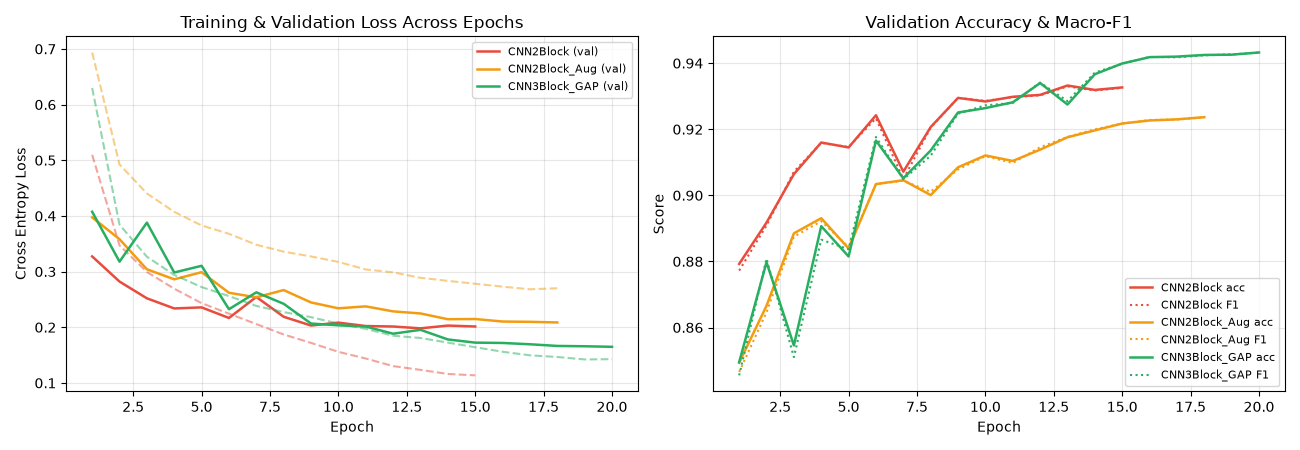
\includegraphics[width=\columnwidth]{cnn_01_training_curves.png}\caption{Loss and validation accuracy curves for the three CNN models.}\label{fig:curves}\end{figure}

\subsection{Statistical Superiority (McNemar Test)}
Paired McNemar tests on the 10{,}000 test predictions confirm that \texttt{CNN3Block-GAP} is statistically superior to \texttt{SVM-RBF (HOG)}:
$$\chi^2 = 44.56, \quad p = 2.46 \times 10^{-11} \ll 0.001$$
The CNN correctly classified 445 images that the SVM failed on, while the SVM was uniquely correct on only 266.

\subsection{Upper-Body Garment Error Resolution}
Total test errors fell from 870 (SVM) down to \textbf{691} (\texttt{CNN3Block-GAP}), eliminating 179 misclassifications:
\begin{itemize}
\item \textbf{Pullover Recall:} 0.856 (SVM) $\to$ \textbf{0.906} (CNN3Block) (+5.0 points).
\item \textbf{Coat Recall:} 0.875 (SVM) $\to$ \textbf{0.924} (CNN3Block) (+4.9 points).
\item \textbf{Shirt Recall:} 0.750 (SVM) $\to$ \textbf{0.763} (CNN3Block).
\end{itemize}

\subsection{Explainability via Grad-CAM}
Grad-CAM heatmaps (Fig.~\ref{fig:gradcam}) on the final convolution layer show that the CNN concentrates attention on the collar neckline (distinguishing T-shirts from open shirts) and hemlines (distinguishing coats from pullovers), explaining why learned representations surpass fixed HOG bins.

\begin{figure*}[t]\centering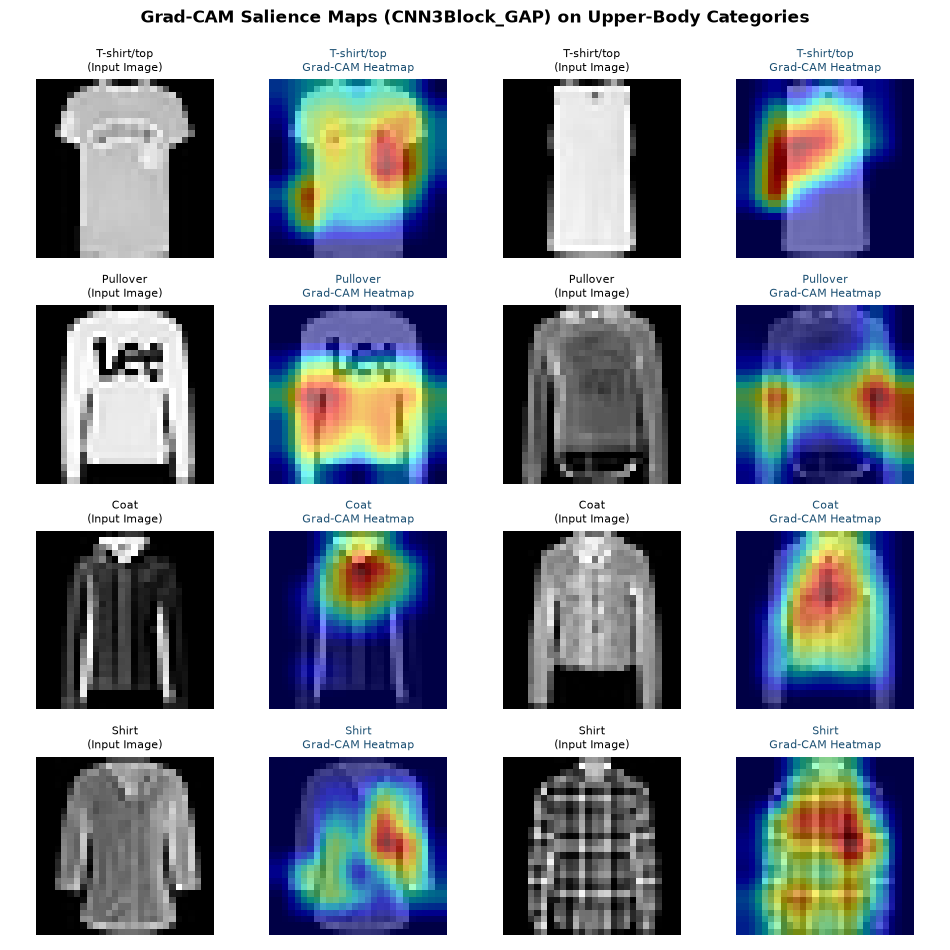
\includegraphics[width=0.92\textwidth]{cnn_02_gradcam_gallery.png}\caption{Grad-CAM saliency heatmaps for upper-body categories under \texttt{CNN3Block-GAP}.}\label{fig:gradcam}\end{figure*}

\section{Conclusion}
Phase~2 demonstrated that end-to-end convolutional networks with Global Average Pooling definitively break the classical machine learning ceiling on Fashion-MNIST, reaching 93.09\% test accuracy ($p = 2.46\times10^{-11}$), reducing model storage by $60\times$, and accelerating CPU inference by $8\times$.

\begin{thebibliography}{99}
\bibitem{xiao2017} H.~Xiao, K.~Rasul, and R.~Vollgraf, ``Fashion-MNIST: a novel image dataset for benchmarking machine learning algorithms,'' arXiv:1708.07747, 2017.
\bibitem{lecun1998} Y.~LeCun, L.~Bottou, Y.~Bengio, and P.~Haffner, ``Gradient-based learning applied to document recognition,'' \emph{Proc. IEEE}, vol.~86, no.~11, pp.~2278--2324, 1998.
\bibitem{selvaraju2017} R.~R. Selvaraju \emph{et al.}, ``Grad-CAM: Visual explanations from deep networks via gradient-based localization,'' in \emph{Proc. IEEE ICCV}, 2017, pp.~618--626.
\end{thebibliography}

\end{document}
